\subsection{Data Normalization and Binning}
\begin{figure}[h]
\centering
    \begin{subfigure}{0.2\textwidth}
        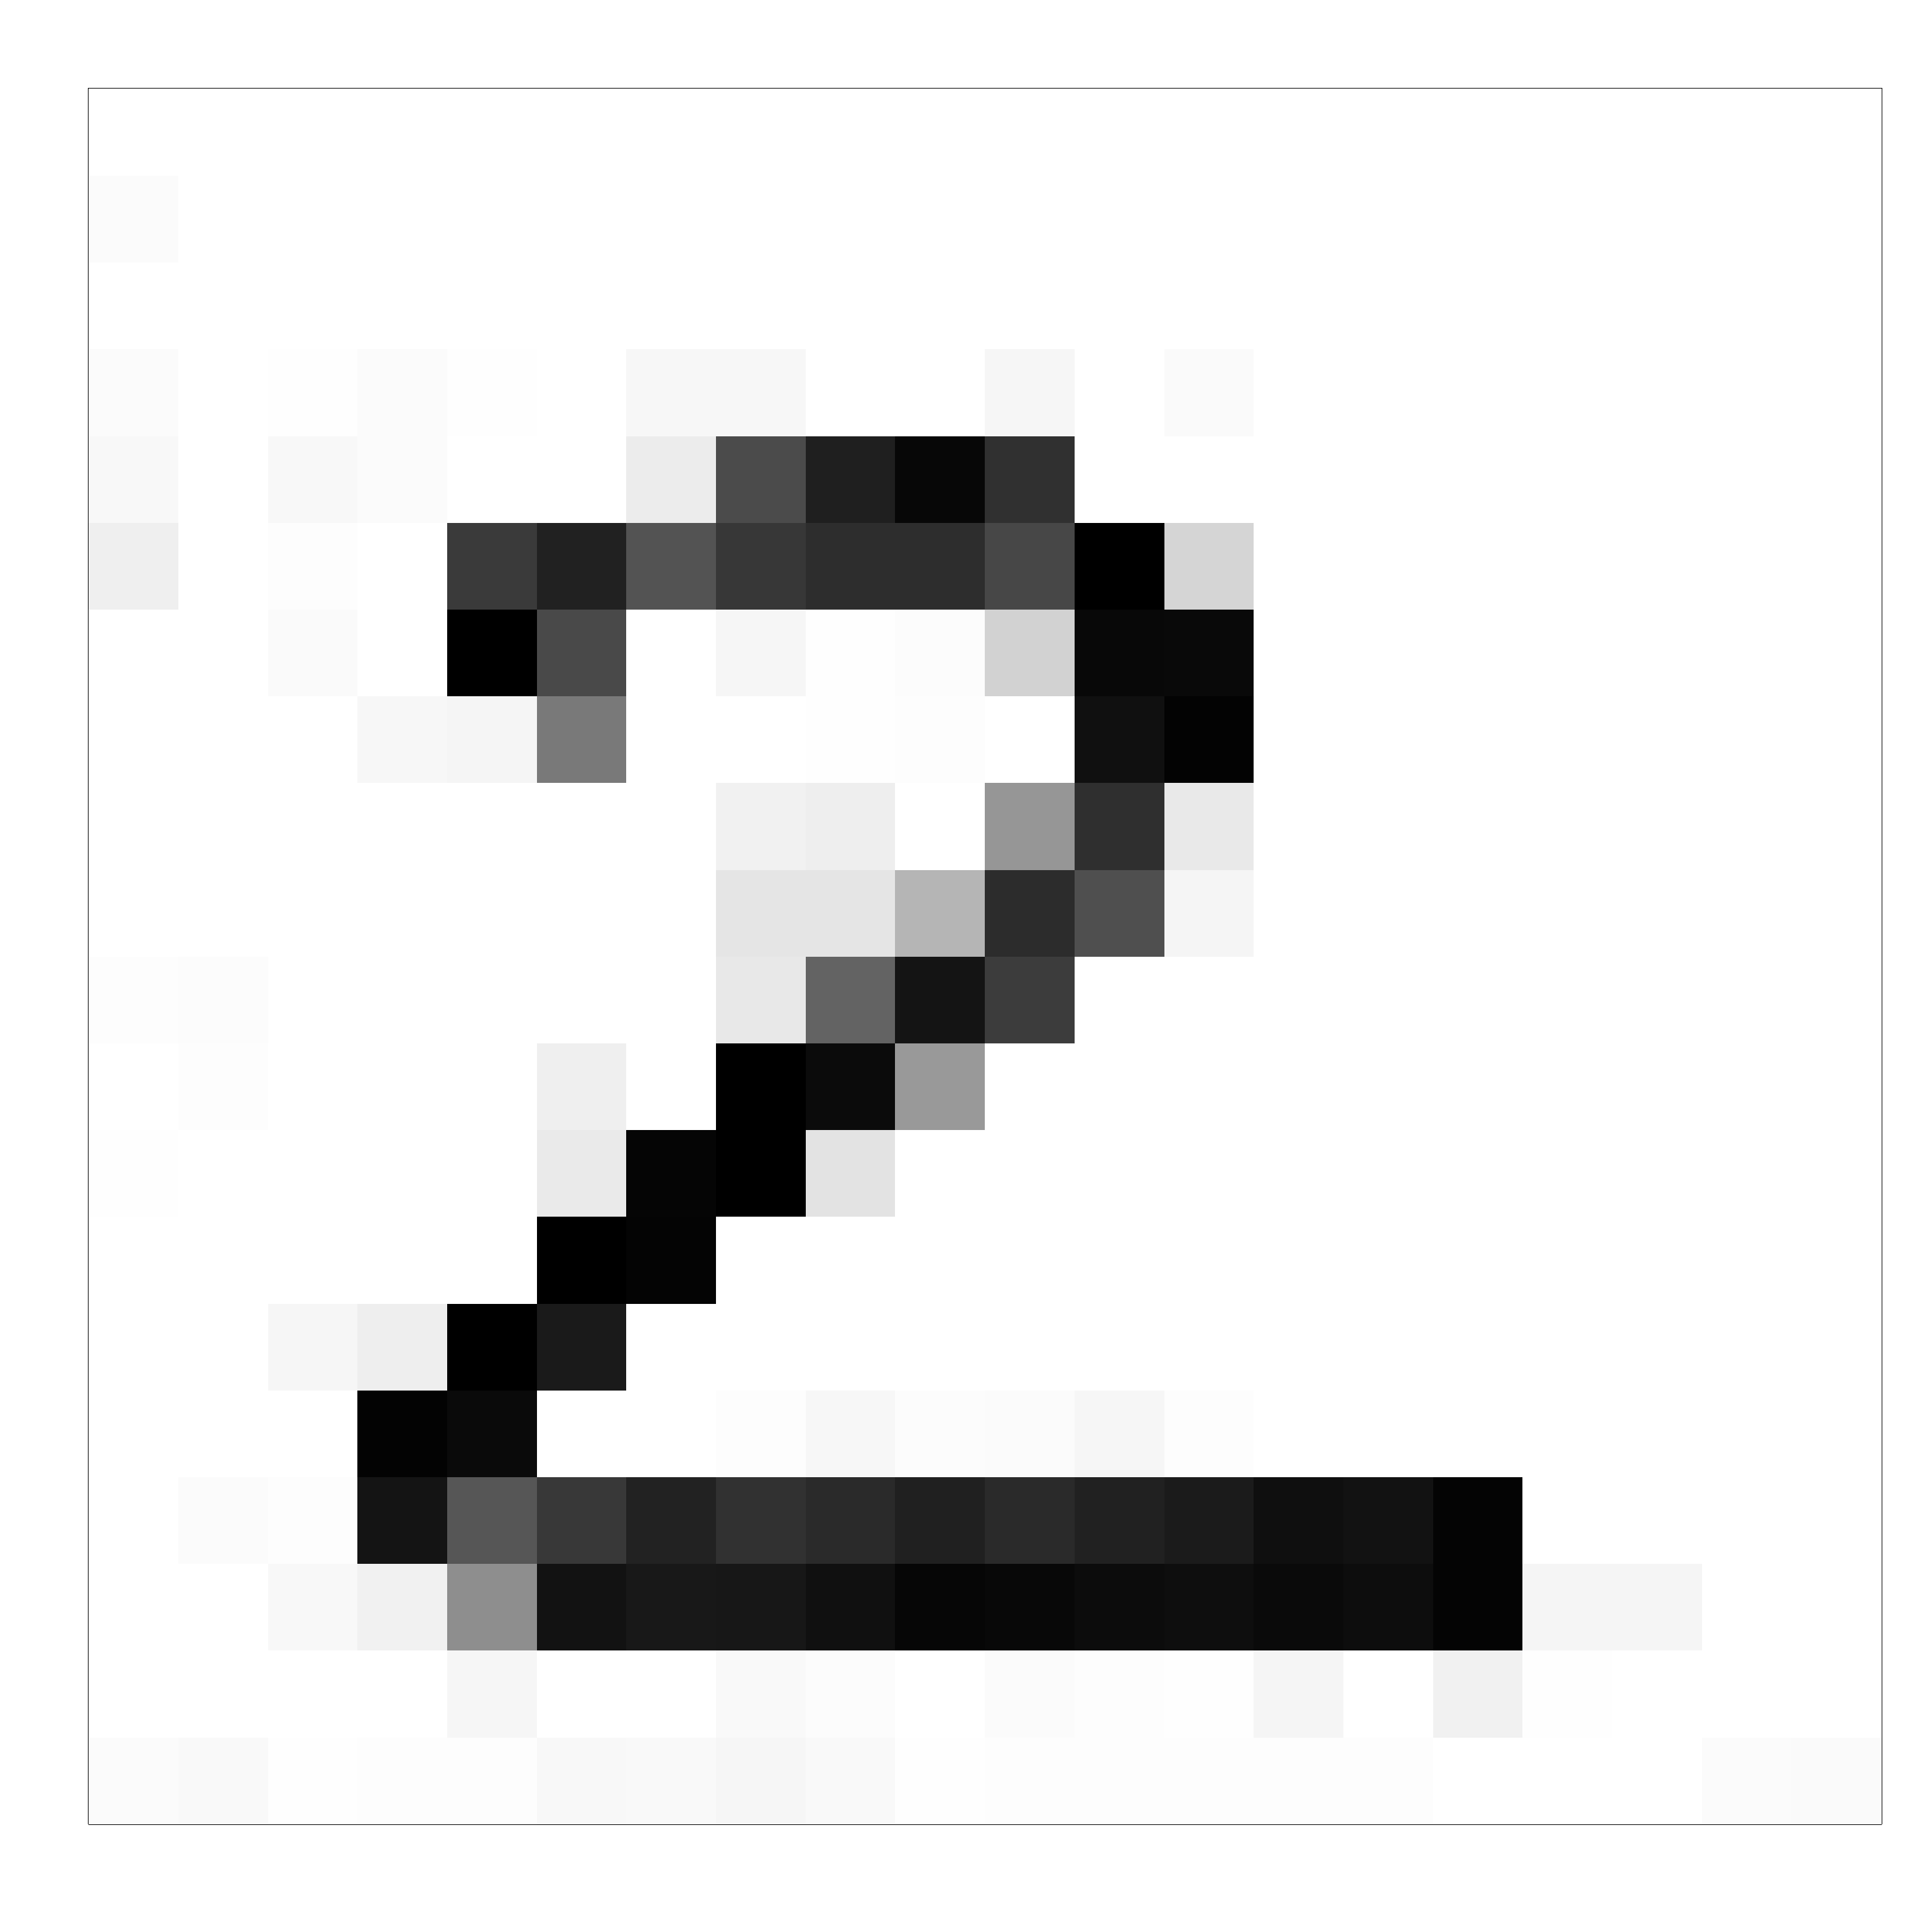
\includegraphics[width = \textwidth]{graphics/bins_inf}
    \end{subfigure}
    \begin{subfigure}{0.2\textwidth}
        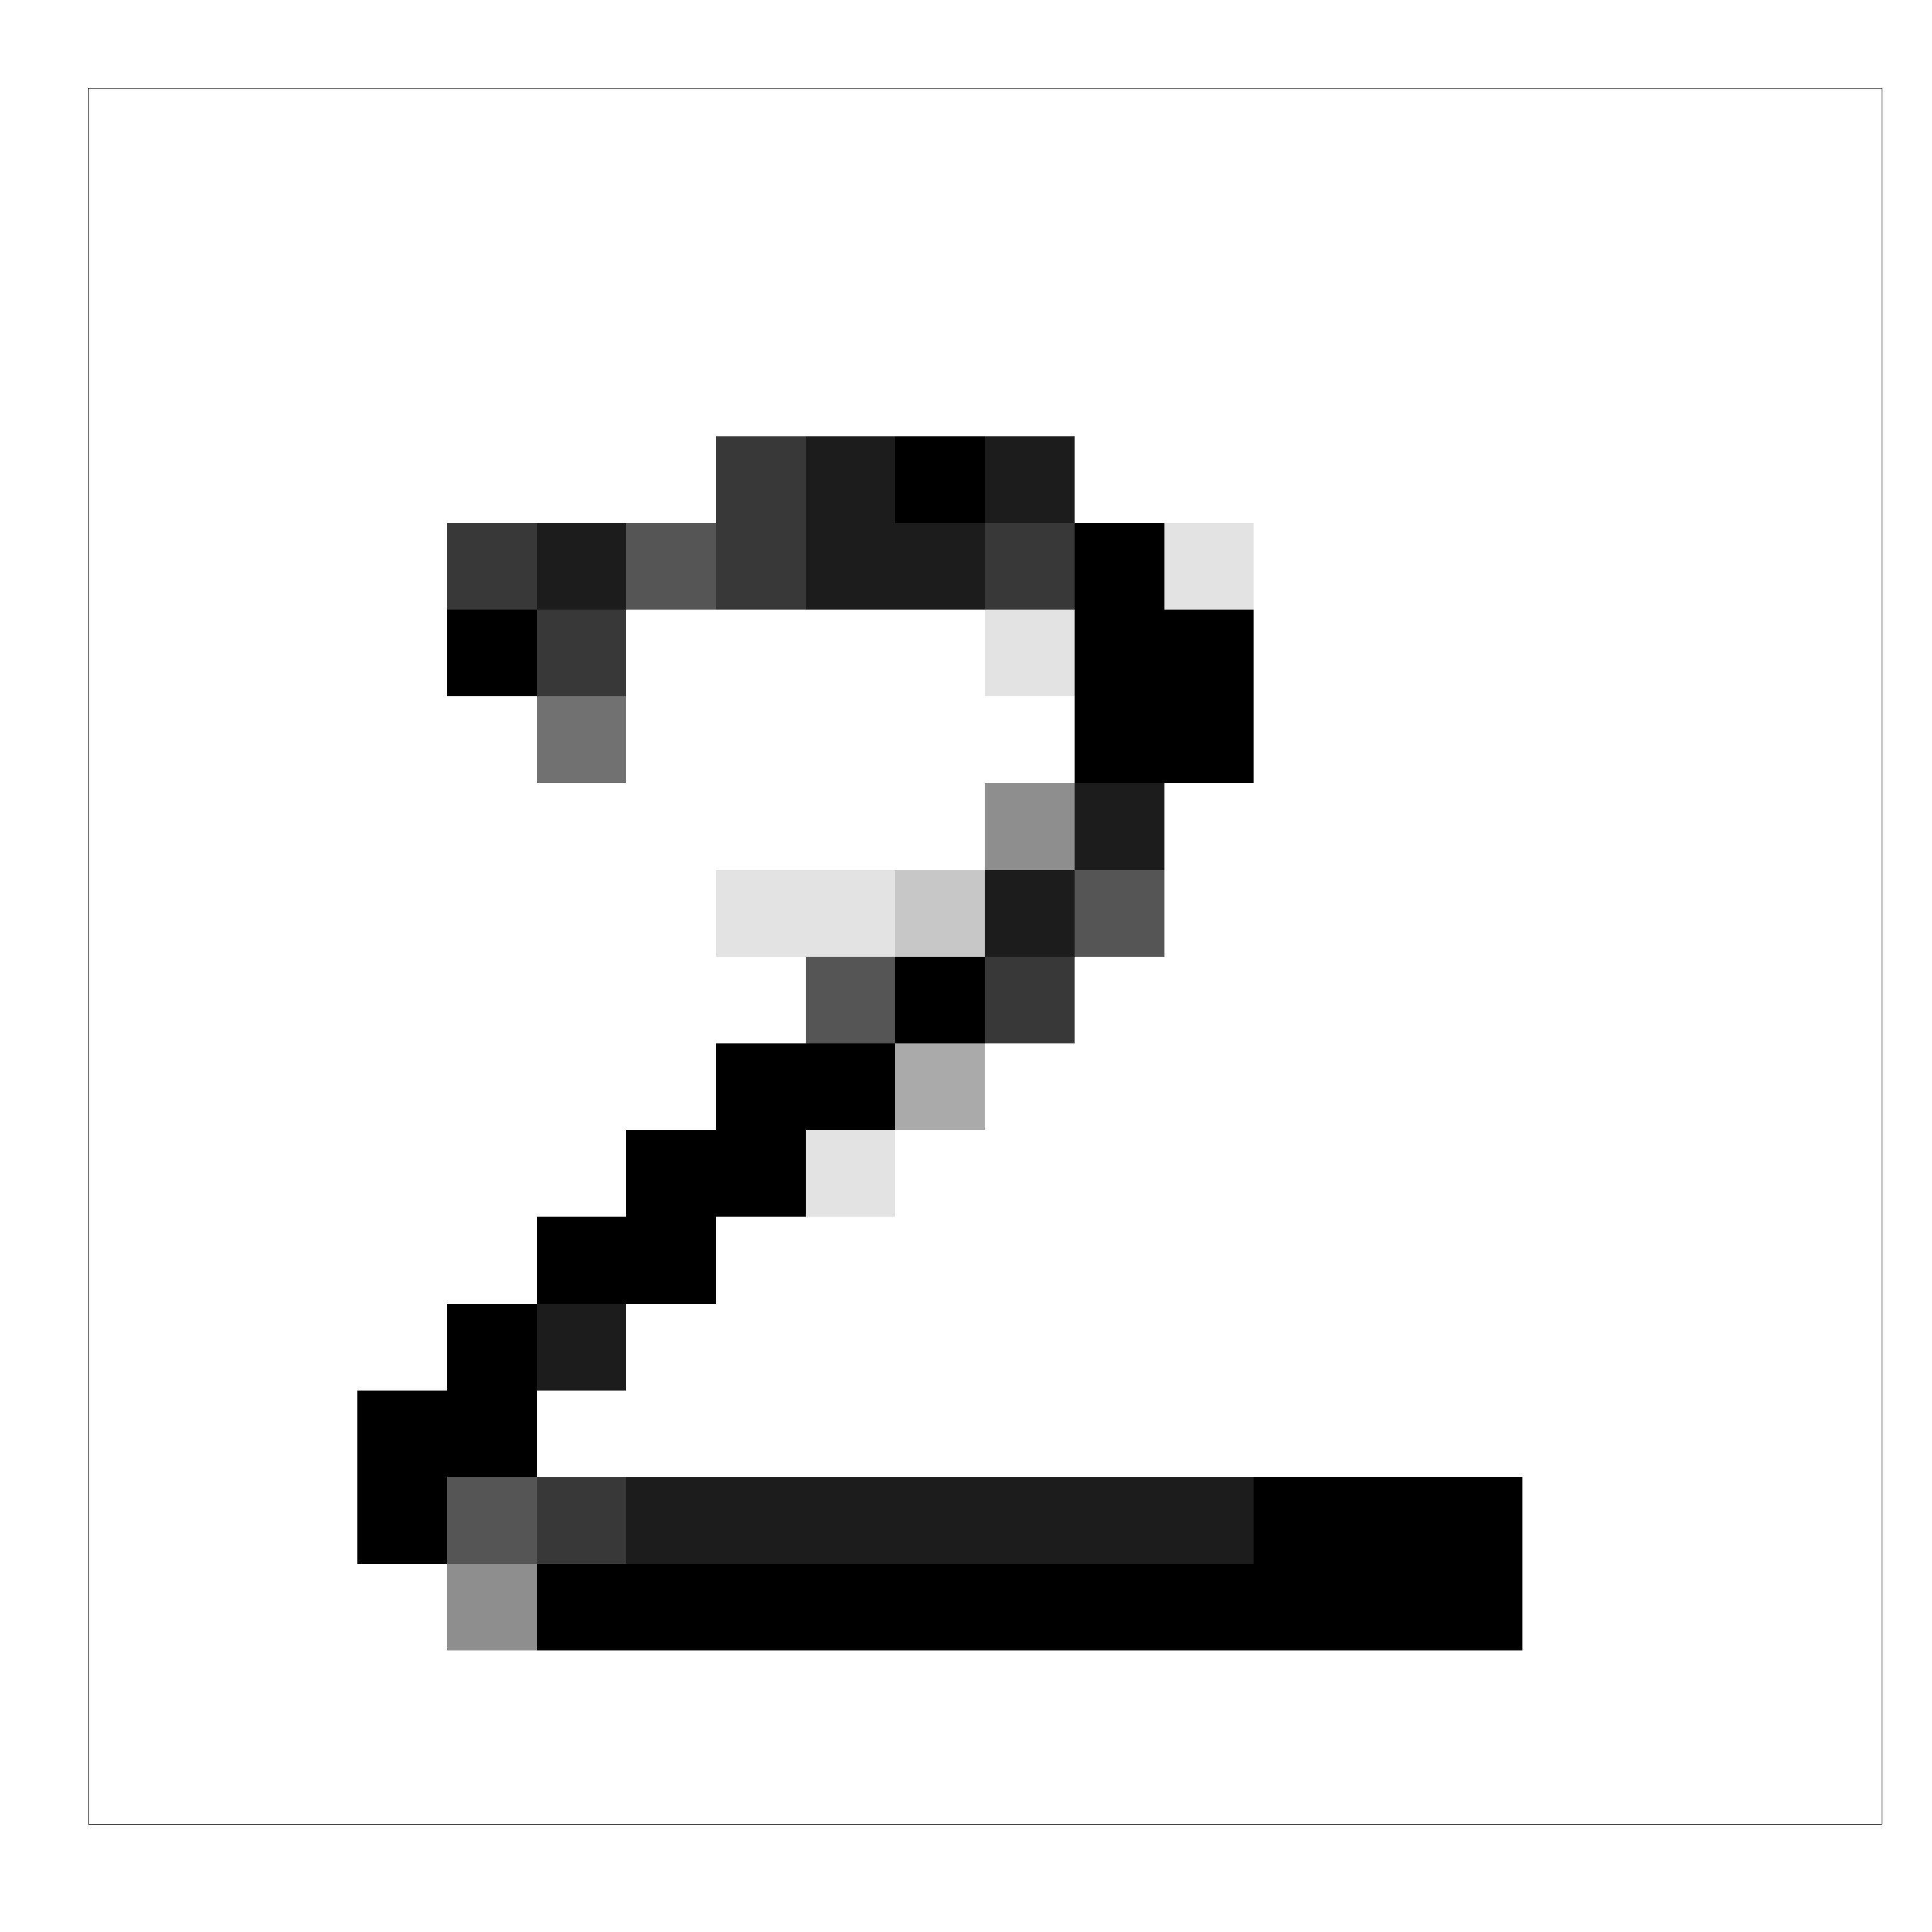
\includegraphics[width = \textwidth]{graphics/bins_10}
    \end{subfigure}
    \begin{subfigure}{0.2\textwidth}
        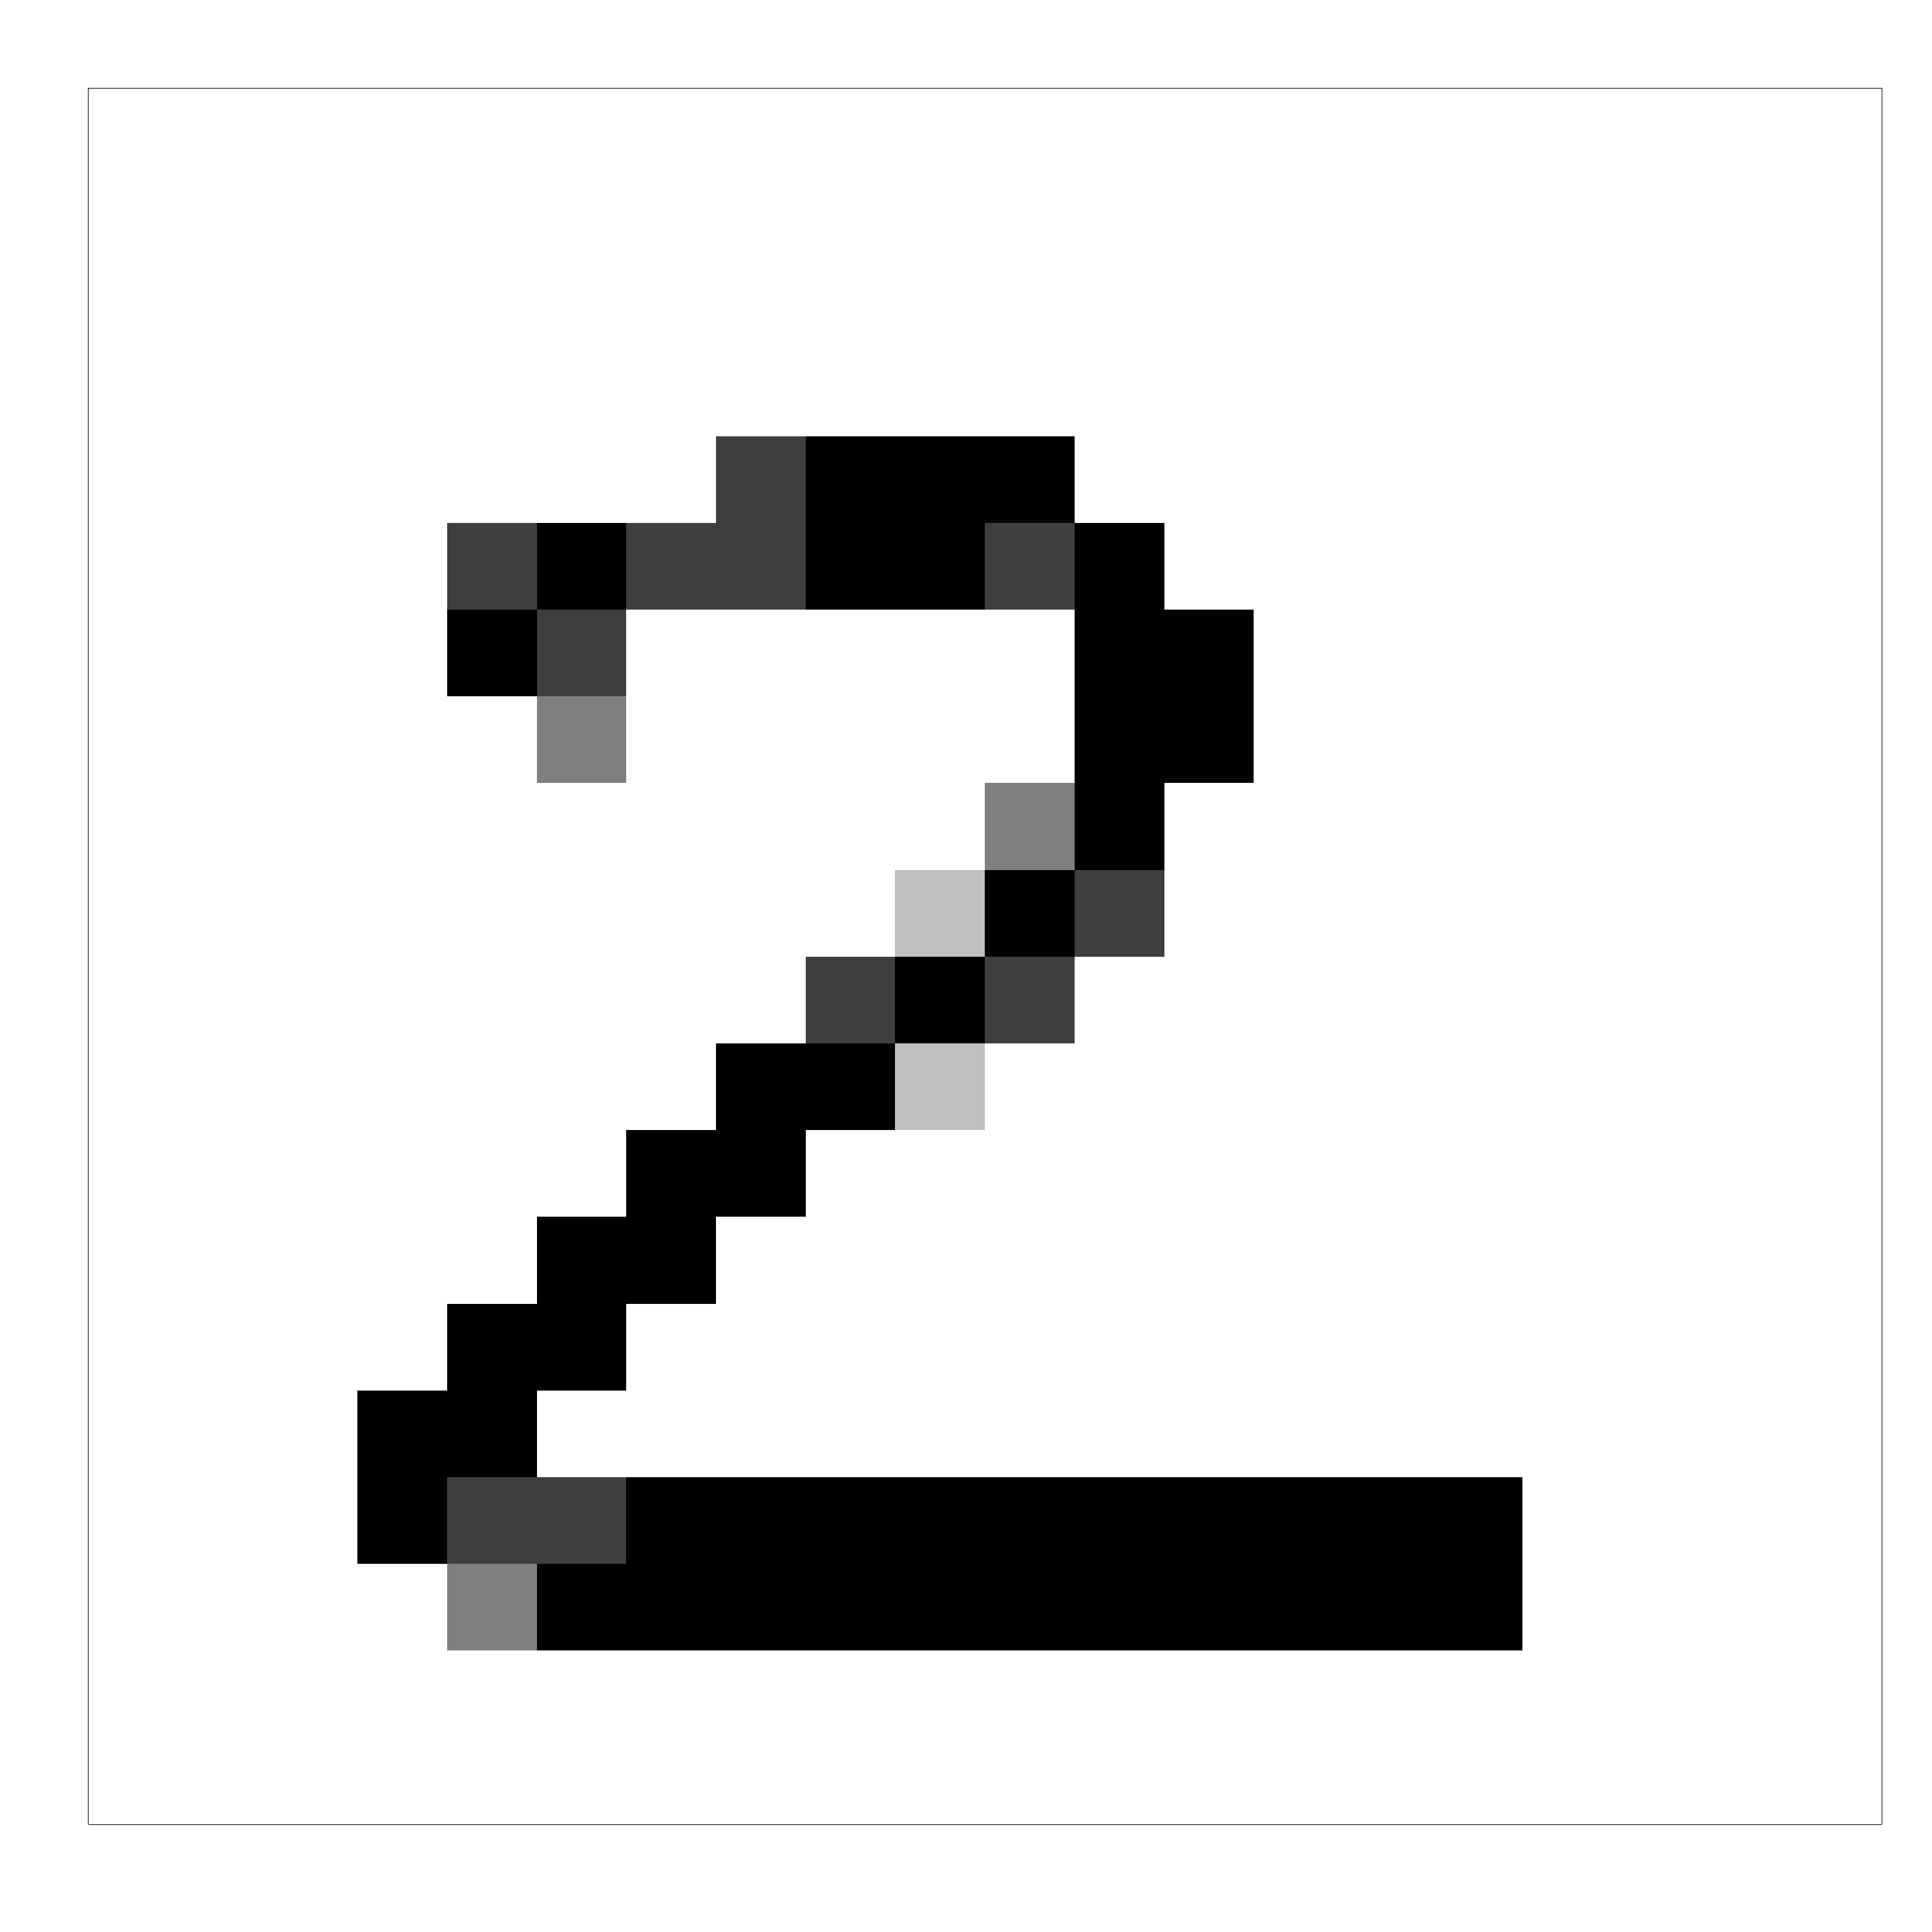
\includegraphics[width = \textwidth]{graphics/bins_5}
    \end{subfigure}
    \begin{subfigure}{0.2\textwidth}
        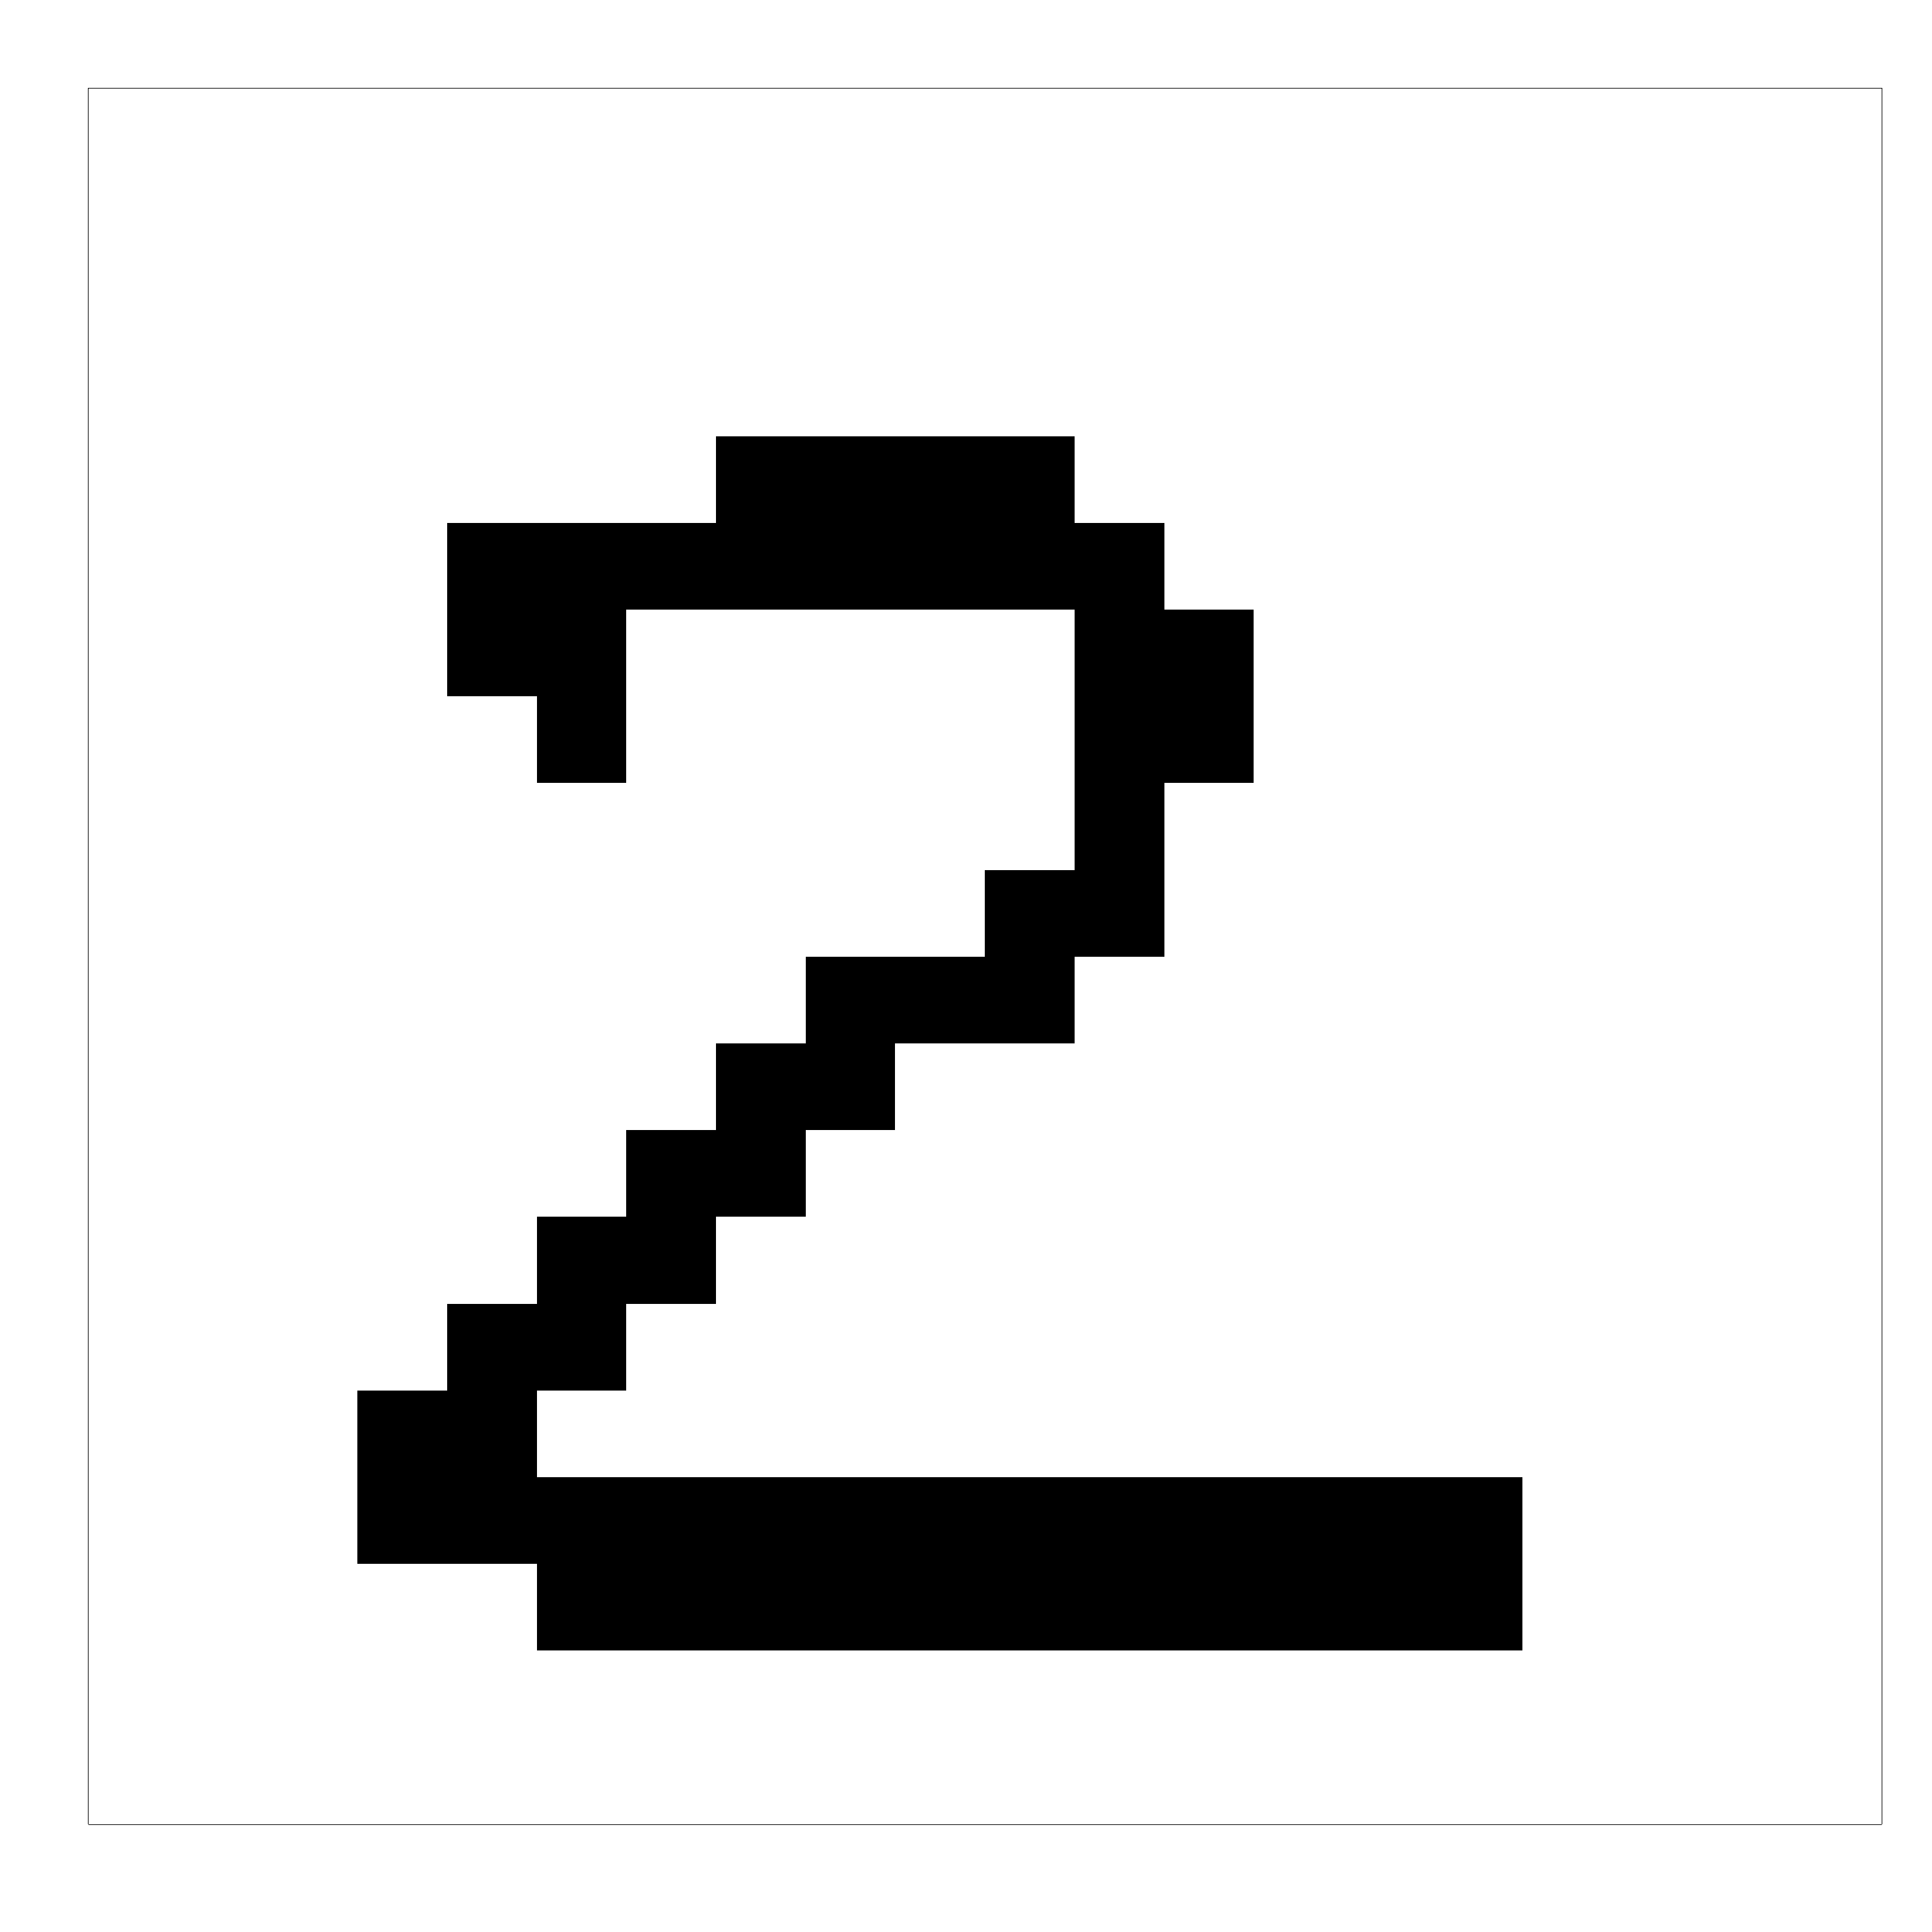
\includegraphics[width = \textwidth]{graphics/bins_2}
    \end{subfigure}
\caption{look at these beautiful 2's}
\end{figure}

To reduce the number of classes to calculate the Naive Bayes for, then the data set is reduced by binning it (grouping it together).
This can be done on various ways:

\begin{itemize}
\item The pixel values can be grouped into 'x' number of groups.
This reduces the probability calculations to be done in the Naive Bayes. \label{list:bin}
\item Nearby pixels can be grouped together, which is the same as reducing the resolution.
\item PCA can be applied on the data to find the most significant variation in the data and step \ref{list:bin} can be applied. \label{list:pca_bin}
\end{itemize}

From these methods, method \ref{list:pca_bin} was chosen.